\subsection{Symbols (\texorpdfstring{$\mathbf s$}{s})}\label{subsec:simbolos}
A symbol represents a group of bits. Modulation defines how each group of bits is converted into a symbol \cite{goldsmith}. In 5G NR, symbols are transmitted within a resource grid, which is formed by subcarriers in the frequency domain and OFDM symbols in the time domain \cite{3gpp-ts38211}.
% FONTE: Goldsmith, p. 127 e pp. 141-142; TS 38.211 v18.6.0, Sec. 4.4.2.

\subsubsection{Modulation}\label{subsubsec:modulacao}
Information bits undergo digital modulation to be transformed into a signal that can be transmitted over a channel. Each group of bits is represented as a point on the complex plane, with an in-phase and a quadrature component. Each point is a symbol, and the set of all such points is called a constellation. In QAM (Quadrature Amplitude Modulation), information is encoded in both amplitude and phase, whereas in PSK (Phase-Shift Keying) it is encoded solely in the phase \cite{goldsmith}.
% FONTE: Goldsmith, p. 127 e pp. 141-142.

The number of points in a constellation determines how many bits each symbol carries. The modulation schemes used in this work, QPSK (Quadrature Phase-Shift Keying) and 16-QAM, have 4 and 16 points, respectively, and carry 2 and 4 bits per symbol (Figure~\ref{fig:constelacoes}). Each symbol is transmitted with an average energy $E_s$ \cite{zhao2025jsac}. The error probability depends on the minimum distance between the points. With the same energy, the points of 16-QAM are closer to each other, so 16-QAM needs a higher SNR than QPSK for the same error probability \cite{tse-viswanath}.
% FONTE: tse-viswanath p. 56 (Eq. 3.24), p. 57 (Fig. 3.3), p. 60 (Tab. 3.1), p. 386 (Eq. 9.12).

\begin{figure}[!ht]
\caption{QPSK and 16-QAM constellations with the same average energy per symbol and the bits of each point.}
\label{fig:constelacoes}
\vspace{4pt}
\centering
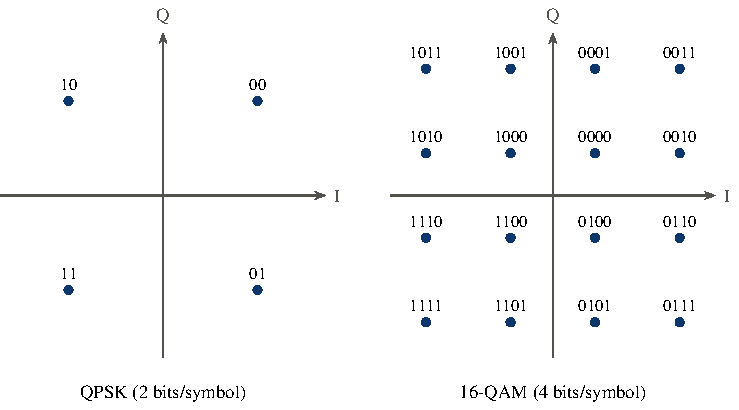
\includegraphics{Images/FLUXO/constelacoes.pdf}
\vspace{4pt}
\legend{Source: adapted from \citesp{goldsmith} and \citesp{3gpp-ts38211}.}
\end{figure}
% FONTE: Goldsmith, Fig. 5.18, p. 149; Tse e Viswanath, p. 57 (Fig. 3.3); TS 38.211 v18.6.0, Secs. 5.1.3 e 5.1.4.

\subsubsection{Resource Grid}\label{subsubsec:grade-recursos}
\textcolor{blue}{These symbols are transmitted in 5G NR using Orthogonal Frequency Division Multiplexing (OFDM), a transmission technique that divides the frequency band into orthogonal subcarriers, each carrying one symbol \cite{tse-viswanath}.} A Resource Element (RE) is one subcarrier during one OFDM symbol. A Resource Block (RB) consists of 12 consecutive subcarriers. The Physical Resource Blocks (PRBs) are the RBs inside the part of the band configured for the transmission, which has from 1 to 275 RBs \cite{3gpp-ts38211, lin-lee-5g}. The number of PRBs in a transmission is denoted as $N_{\text{PRB}}$. Since the receiver processes each PRB, $N_{\text{PRB}} = 275$ is the worst case for 5G NR \cite{zhao2025jsac}.
% FONTE: Tse e Viswanath, Seção 3.4.4, p. 99; TS 38.211 Secs. 4.4.3, 4.4.4.1 e 4.4.4.4; Lin e Lee, p. 367; zhao2025jsac paper.md:640.

In the time domain, OFDM symbols are grouped into slots, each containing 14 symbols. The data of the User Equipments (UEs) is transmitted on the Physical Uplink Shared Channel (PUSCH) \cite{3gpp-ts38211}. A UE transmits the PUSCH only in the slots that the base station assigns to it. In Time Division Duplex (TDD), the uplink and the downlink use the same frequency band, but at different times \cite{lin-lee-5g}. \textcolor{blue}{Therefore, only the uplink slots can carry the PUSCH in TDD.}
% FONTE: Lin e Lee, pp. 104 e 293; TS 38.211 Tab. 4.3.2-1 e Sec. 6.3.1.
